\documentclass[aspectratio=169,11pt]{beamer}

\usepackage[T1]{fontenc}
\usepackage[utf8]{inputenc}
\usepackage{lmodern}
\usepackage{amsmath,amssymb}
\usepackage{booktabs}
\usepackage{tikz}
\usetikzlibrary{arrows.meta,positioning}

\definecolor{accent}{RGB}{30,74,118}
\definecolor{memberred}{RGB}{178,56,56}
\definecolor{softbg}{RGB}{236,242,248}
\definecolor{softred}{RGB}{251,238,238}
\definecolor{graytext}{RGB}{110,115,120}

\setbeamertemplate{navigation symbols}{}
\setbeamercolor{structure}{fg=accent}
\setbeamercolor{title}{fg=accent}
\setbeamercolor{frametitle}{fg=accent}
\setbeamercolor{block title}{bg=accent,fg=white}
\setbeamercolor{block body}{bg=softbg,fg=black}
\setbeamerfont{title}{size=\LARGE,series=\bfseries}
\setbeamerfont{frametitle}{size=\Large,series=\bfseries}

\setbeamertemplate{footline}{%
  \leavevmode\hbox{%
    \hspace*{0.7cm}{\footnotesize\color{graytext}Money-Laundering Ring Detection\quad\insertframenumber/\inserttotalframenumber}%
  }\vspace*{0.28cm}%
}

\newcommand{\memberbadge}[1]{%
  \hfill{\small\bfseries\color{memberred}#1}%
}

\begin{document}

% ========================== SLIDE 1 ==========================
\begin{frame}[plain]
\centering
\vspace*{1.0cm}
{\LARGE\bfseries\color{accent} Money-Laundering Ring Detection\\[0.2cm] with Graph Algorithms\par}
\vspace{0.35cm}
{\large\color{accent} MFCS Group Project\par}

\vspace{0.9cm}
{\normalsize
\begin{tabular}{cccc}
\textbf{Adityaa Saha} & \textbf{Debtanu Das} & \textbf{Jeeban Jyoti Patra} & \textbf{Shatadeep De} \\
{\footnotesize\color{graytext}23CS01002} & {\footnotesize\color{graytext}23CS01016} & {\footnotesize\color{graytext}23CS01026} & {\footnotesize\color{graytext}23CS01072}
\end{tabular}
\par}

\vspace{0.8cm}
{\small IIT Bhubaneswar\par}
\vspace{0.3cm}
{\normalsize November 2026\par}
\end{frame}

% ========================== SLIDE 2 ==========================
\begin{frame}{The problem}
\begin{columns}[T,onlytextwidth]
\begin{column}{0.56\textwidth}
\begin{itemize}
\setlength{\itemsep}{0.6em}
\item Input: a log of bank transfers (time, sender, receiver, amount, label).
\item Goal: flag the transfers that form \textbf{laundering patterns}.
\item Data: IBM synthetic AML data set (eleven columns, ``Is Laundering'' label).
\item \textbf{Graph theory only}: no ML. Each detector has a definition, a proof and a complexity bound.
\end{itemize}
\end{column}
\begin{column}{0.42\textwidth}
\centering
\vspace{0.4cm}
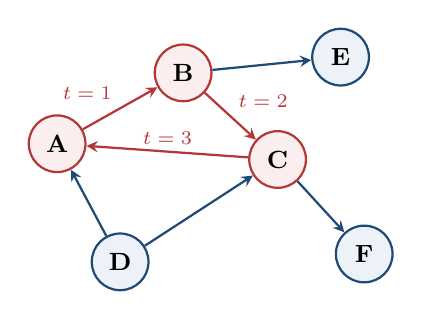
\begin{tikzpicture}[
    cyc/.style={circle, draw=memberred, thick, fill=softred, minimum size=0.72cm, font=\small\bfseries},
    oth/.style={circle, draw=accent, thick, fill=softbg, minimum size=0.72cm, font=\small\bfseries},
    cyce/.style={->, >=stealth, thick, color=memberred},
    othe/.style={->, >=stealth, thick, color=accent}
]
\node[cyc] (A) at (0,0) {A};
\node[cyc] (B) at (1.6,0.9) {B};
\node[cyc] (C) at (2.8,-0.2) {C};
\node[oth] (D) at (0.8,-1.5) {D};
\node[oth] (E) at (3.6,1.1) {E};
\node[oth] (F) at (3.9,-1.4) {F};

\draw[cyce] (A) -- node[above left=-1pt,font=\scriptsize] {$t=1$} (B);
\draw[cyce] (B) -- node[above right=-1pt,font=\scriptsize] {$t=2$} (C);
\draw[cyce] (C) -- node[above=-1pt,font=\scriptsize] {$t=3$} (A);
\draw[othe] (B) -- (E);
\draw[othe] (D) -- (A);
\draw[othe] (D) -- (C);
\draw[othe] (C) -- (F);
\end{tikzpicture}

\vspace{0.3cm}
{\footnotesize accounts = vertices, transfers = timed edges}
\end{column}
\end{columns}
\end{frame}

% ========================== SLIDE 3 ==========================
\begin{frame}{Graph model and detection pipeline}
\textbf{Graph model:} directed temporal multigraph $G = (V, E)$ with amount $a(e)$ and time $t(e)$. Dense detectors use the simple undirected projection $H$, with density $\rho(S) = |E(S)| / |S|$.

\vspace{0.15cm}
\centering
{\scriptsize
\setlength{\tabcolsep}{3.5pt}
\begin{tabular}{@{}lll@{}}
\toprule
\textbf{Pipeline Stage} & \textbf{Core Algorithm \& Guarantee} & \textbf{Detection Target} \\
\midrule
\textbf{1. Ingestion \& SCC} & Stable sort, Kosaraju SCC & Time-ordered lists, SCC pruning \\
\textbf{2. Temporal Patterns} & Pruned window DFS, sliding window & Temporal cycles ($2..K$), smurfing hubs \\
\textbf{3. Layering \& Peeling} & DAG DP, Charikar greedy peeling & Pass-through chains, dense cores \\
\textbf{4. Exact Densest \& Eval} & Min-cut reduction + Dinkelbach & Exact densest ring $\rho^*$, evaluation \\
\bottomrule
\end{tabular}
}

\vspace{0.3cm}
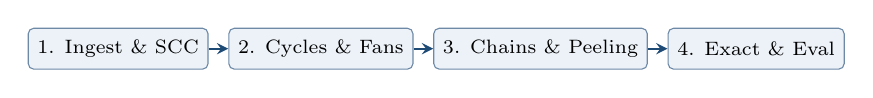
\begin{tikzpicture}[
    box/.style={draw=accent!65, fill=softbg, rounded corners=2pt, font=\scriptsize, minimum width=2.2cm, minimum height=0.52cm, align=center},
    arr/.style={->, >=stealth, thick, color=accent}
]
\node[box] (s1) {1. Ingest \& SCC};
\node[box, right=0.25cm of s1] (s2) {2. Cycles \& Fans};
\node[box, right=0.25cm of s2] (s3) {3. Chains \& Peeling};
\node[box, right=0.25cm of s3] (s4) {4. Exact \& Eval};
\draw[arr] (s1) -- (s2);
\draw[arr] (s2) -- (s3);
\draw[arr] (s3) -- (s4);
\end{tikzpicture}

\vspace{0.15cm}
{\footnotesize one program: \texttt{clang++ -std=c++17 -O2 src/exact\_eval.cpp -o aml}}
\end{frame}

% ========================== SLIDE 4 ==========================
\begin{frame}{Ingestion and the graph \memberbadge{Adityaa Saha}}
\begin{itemize}
\setlength{\itemsep}{0.45em}
\item Parse the eleven IBM columns, with portable hand-written epoch conversion.
\item Accounts ``bank:account'' are mapped to integers $0\dots n-1$ through a hash map.
\item Parallel edges and self loops are kept. Malformed rows are skipped and counted.
\item \texttt{finalize()}: stable sort by time, then fill $\text{out}(u)$ and $\text{in}(u)$ in one scan. Cost $O(m \log m)$.
\end{itemize}

\vspace{0.35cm}
\begin{block}{Invariant: time-sorted adjacency}
Every adjacency list is in non-decreasing time order, because it is filled in increasing index order from a time-sorted array. So ``edges of $u$ after time $\tau$'' is a binary search, which downstream pattern detectors rely on.
\end{block}
\end{frame}

% ========================== SLIDE 5 ==========================
\begin{frame}{Kosaraju's SCC algorithm \memberbadge{Adityaa Saha}}
\begin{columns}[T,onlytextwidth]
\begin{column}{0.58\textwidth}
\begin{itemize}
\setlength{\itemsep}{0.55em}
\item DFS assigns $\text{disc}[v]$ and pushes $v$ on a stack.
\item $\text{low}[v]$ is the smallest $\text{disc}$ of a stack vertex reachable from $T(v)$.
\item When $v$ finishes with $\text{low}[v] = \text{disc}[v]$, pop one SCC.
\item \textbf{Iterative} with an explicit stack: a 200\,000-vertex path does not overflow.
\item Cost $O(n + m)$.
\end{itemize}
\end{column}
\begin{column}{0.39\textwidth}
\vspace{0.2cm}
\begin{block}{Why we need it}
A cycle lives inside one SCC.\\
Cycle detection prunes every search edge that leaves the root's SCC.
\end{block}
\end{column}
\end{columns}
\end{frame}

% ========================== SLIDE 6 ==========================
\begin{frame}{Kosaraju 2-pass SCC \memberbadge{Adityaa Saha}}
\textbf{Theorem.} When $v$ finishes, $\text{low}[v] = \text{disc}[v] \iff v$ is the root of its SCC, and the popped set is exactly that SCC.

\vspace{0.3cm}
\begin{itemize}
\setlength{\itemsep}{0.55em}
\item \textbf{Facts.} (A) The active vertices form the DFS path. (B) An SCC lies in its root's subtree. (S) A vertex is on the stack iff its SCC's root is unfinished.
\item \textbf{Not root $\Rightarrow \text{low} < \text{disc}$.} The root $r$ is a proper ancestor. On a path $v \rightsquigarrow r$, the first edge leaving $T(v)$ hits $y$ with $\text{disc}[y] < \text{disc}[v]$, and $y$ is on the stack by (S).
\item \textbf{$\text{low} < \text{disc} \Rightarrow$ not root.} A reachable stack vertex $w$ has an unfinished root $r'$, which is a proper ancestor. So $v \to w \to r' \to v$.
\item \textbf{Popped set.} Vertices above $v$ lie in $T(v)$, and their root must be $v$. All of $v$'s SCC is still there by (B) and (S).
\end{itemize}
\end{frame}

% ========================== SLIDE 7 ==========================
\begin{frame}{Ingestion and SCC: verification \memberbadge{Adityaa Saha}}
\begin{itemize}
\setlength{\itemsep}{0.5em}
\item Hand-made CSV: parallel edges, a self loop, rows out of order, a malformed row. Checks degrees, the handshake sum, the sorted invariant and the Amount Paid column.
\item Timestamps: the epoch, a leap day, a wrong format.
\item \textbf{1000 random graphs}: Kosaraju's components match mutual reachability from a transitive closure.
\item A 200\,000-vertex cycle gives exactly one SCC, with no stack overflow.
\item Synthetic generator round trip: every planted transfer comes back labelled.
\end{itemize}

\vspace{0.35cm}
\centering
\colorbox{softbg}{\texttt{[ingest\_scc] ingestion + SCC tests: PASS}}
\end{frame}

% ========================== SLIDE 8 ==========================
\begin{frame}{Temporal cycles: definition \memberbadge{Debtanu Das}}
\begin{columns}[T,onlytextwidth]
\begin{column}{0.60\textwidth}
A \textbf{temporal cycle} $e_1, \dots, e_k$ with $2 \le k \le K$:
\begin{enumerate}
\setlength{\itemsep}{0.25em}
\item head-to-tail, closing back at the start;
\item distinct vertices;
\item $t(e_1) \le \dots \le t(e_k)$;
\item $t(e_k) - t(e_1) \le W$;
\item $e_1$ has the smallest index (one representative per cycle).
\end{enumerate}
\vspace{0.2cm}
\textbf{Search:} from each edge $r$, run a DFS of depth $\le K$, scanning out-edges in time order. Stop past $t(r) + W$, skip indices $\le r$, and stay inside the SCC.
\end{column}
\begin{column}{0.36\textwidth}
\centering
\vspace{0.8cm}
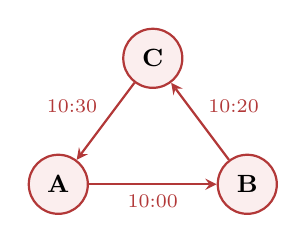
\begin{tikzpicture}[
    v/.style={circle, draw=memberred, thick, fill=softred, minimum size=0.75cm, font=\small\bfseries},
    e/.style={->, >=stealth, thick, color=memberred}
]
\node[v] (A) at (0,0) {A};
\node[v] (B) at (2.4,0) {B};
\node[v] (C) at (1.2,1.6) {C};
\draw[e] (A) -- node[below,font=\scriptsize] {10:00} (B);
\draw[e] (B) -- node[above right=-1pt,font=\scriptsize] {10:20} (C);
\draw[e] (C) -- node[above left=-1pt,font=\scriptsize] {10:30} (A);
\end{tikzpicture}

\vspace{0.3cm}
{\footnotesize round-tripping within $W$}
\end{column}
\end{columns}
\end{frame}

% ========================== SLIDE 9 ==========================
\begin{frame}{Proof: the bounded search is exact \memberbadge{Debtanu Das}}
\textbf{Lemma.} All vertices of a temporal cycle share one SCC (a closed walk), so SCC pruning loses nothing.

\vspace{0.25cm}
\textbf{Theorem.} (a) Every output has $2..K$ edges and the search terminates. (b) Every output is a temporal cycle. (c) Every temporal cycle is output \emph{exactly once}.
\begin{itemize}
\setlength{\itemsep}{0.35em}
\item (a) A path is extended only while $|P| + 1 < K$, and the depth is $\le K$.
\item (b) Each of conditions 1--5 is enforced by one check: the adjacency list, the on-path marks, $t \ge \tau$, the deadline, and the index skip.
\item (c) Root the search at $e_1$. By induction, each $e_{i+1}$ passes every check. Uniqueness: by condition 5, only the search rooted at $e_1$ can produce the cycle.
\end{itemize}

\vspace{0.25cm}
\textbf{Cost} $O(m\,d^{K-1})$, where $d$ is the maximum out-degree inside a window. This is exponential in $K$, so $K$ must be bounded.
\end{frame}

% ========================== SLIDE 10 ==========================
\begin{frame}{Fan-out / fan-in (smurfing) \memberbadge{Debtanu Das}}
\begin{columns}[T,onlytextwidth]
\begin{column}{0.58\textwidth}
\begin{itemize}
\setlength{\itemsep}{0.45em}
\item Centre $u$ sends to (or receives from) at least $k$ \textbf{distinct} accounts within $W$.
\item Two-pointer sliding window over the time-sorted list, with a counter per counterparty.
\end{itemize}

\vspace{0.3cm}
\begin{block}{Claim: exact, $O(n + m)$}
For each right end, the window kept is the \emph{longest} run spanning at most $W$. Distinct counts only grow with the run, so it qualifies iff any run does. Each pointer moves at most $\deg(u)$ times.
\end{block}
\end{column}
\begin{column}{0.38\textwidth}
\centering
\vspace{0.4cm}
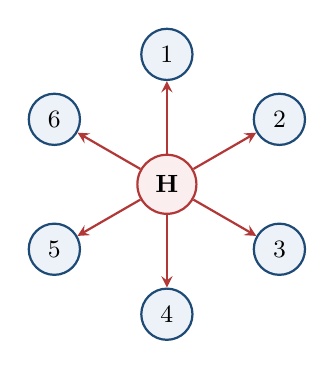
\begin{tikzpicture}[
    hub/.style={circle, draw=memberred, thick, fill=softred, minimum size=0.75cm, font=\small\bfseries},
    leaf/.style={circle, draw=accent, thick, fill=softbg, minimum size=0.65cm, font=\small},
    arr/.style={->, >=stealth, thick, color=memberred}
]
\node[hub] (H) at (0,0) {H};
\foreach \i/\ang in {1/90, 2/30, 3/-30, 4/-90, 5/-150, 6/150} {
    \node[leaf] (N\i) at (\ang:1.65cm) {\i};
    \draw[arr] (H) -- (N\i);
}
\end{tikzpicture}

\vspace{0.25cm}
{\footnotesize one account splits money into many small transfers}
\end{column}
\end{columns}
\end{frame}

% ========================== SLIDE 11 ==========================
\begin{frame}{Cycles and smurfing: verification \memberbadge{Debtanu Das}}
\begin{itemize}
\setlength{\itemsep}{0.55em}
\item Hand-made 3-cycle plus a late parallel edge: exactly 1 cycle at $W = 100\,\text{s}$ and 2 at $W = 480\,\text{s}$. $K = 2$ finds none, and $W = 19$ versus $W = 20$ is the exact boundary.
\item \textbf{400 random graphs}: the cycle set equals an exhaustive enumeration of all edge sequences (345 cycles, no duplicates).
\item Hub-and-sink graph: the window boundaries ($29\,\text{s}$ versus $30\,\text{s}$) and the distinct-counterparty rule.
\item \textbf{2000 random graphs}: the fans match a brute force over all $(i, j)$ windows (6870 centres).
\end{itemize}

\vspace{0.35cm}
\centering
\colorbox{softbg}{\texttt{[cycles\_fan] cycle + fan tests: PASS}}
\end{frame}

% ========================== SLIDE 12 ==========================
\begin{frame}{Pass-through chains (layering) \memberbadge{Jeeban Jyoti Patra}}
\begin{columns}[T,onlytextwidth]
\begin{column}{0.58\textwidth}
$f$ \textbf{follows} $e$: $f$ leaves the account $e$ entered, comes later in index order, within $D$ seconds, and keeps the amount within a $1 - \varepsilon$ factor.

\vspace{0.25cm}
\textbf{DP:} $\text{back}[e]$ is the longest chain ending at $e$ and $\text{fwd}[e]$ the longest starting at $e$. Flag $e$ iff $\text{back} + \text{fwd} - 1 \ge L$.

\vspace{0.3cm}
\begin{block}{Claim: the DP is exact}
``Follows'' is a DAG in index order, and chains only constrain consecutive edges, so the best prefix joined to the best suffix is a chain.
\end{block}
\end{column}
\begin{column}{0.39\textwidth}
\centering
\vspace{1.2cm}
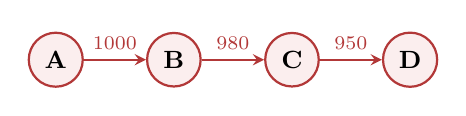
\begin{tikzpicture}[
    v/.style={circle, draw=memberred, thick, fill=softred, minimum size=0.68cm, font=\small\bfseries},
    e/.style={->, >=stealth, thick, color=memberred}
]
\node[v] (A) at (0,0) {A};
\node[v] (B) at (1.5,0) {B};
\node[v] (C) at (3.0,0) {C};
\node[v] (D) at (4.5,0) {D};
\draw[e] (A) -- node[above,font=\scriptsize] {1000} (B);
\draw[e] (B) -- node[above,font=\scriptsize] {980} (C);
\draw[e] (C) -- node[above,font=\scriptsize] {950} (D);
\end{tikzpicture}

\vspace{0.35cm}
{\footnotesize each hop forwards almost everything, quickly}
\end{column}
\end{columns}
\end{frame}

% ========================== SLIDE 13 ==========================
\begin{frame}{$k$-core and Charikar's greedy peeling \memberbadge{Jeeban Jyoti Patra}}
\begin{itemize}
\setlength{\itemsep}{0.5em}
\item Project to the simple undirected graph $H$, where parallel and reverse transfers collapse.
\item Repeatedly delete a \textbf{minimum-degree} vertex, and remember the densest remaining set.
\item A priority queue (std::set) maintains vertices by degree. The same pass gives every core number.
\end{itemize}

\vspace{0.45cm}
\centering
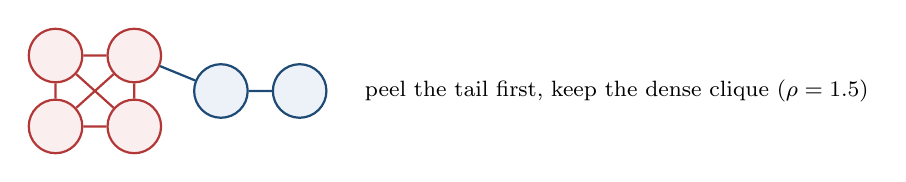
\begin{tikzpicture}[
    clq/.style={circle, draw=memberred, thick, fill=softred, minimum size=0.68cm},
    tail/.style={circle, draw=accent, thick, fill=softbg, minimum size=0.68cm},
    ec/.style={thick, color=memberred},
    et/.style={thick, color=accent}
]
\node[clq] (1) at (0,0.9) {};
\node[clq] (2) at (1.0,0.9) {};
\node[clq] (3) at (0,0) {};
\node[clq] (4) at (1.0,0) {};
\node[tail] (5) at (2.1,0.45) {};
\node[tail] (6) at (3.1,0.45) {};
\draw[ec] (1)--(2)--(4)--(3)--(1)--(4) (2)--(3);
\draw[et] (2)--(5)--(6);
\node[right=0.35cm of 6, font=\footnotesize] {peel the tail first, keep the dense clique ($\rho = 1.5$)};
\end{tikzpicture}
\end{frame}

% ========================== SLIDE 14 ==========================
\begin{frame}{Proof: greedy is a $\frac{1}{2}$-approximation \memberbadge{Jeeban Jyoti Patra}}
Let $S^*$ be densest, with $\rho^* = \rho(S^*)$.

\vspace{0.25cm}
\textbf{Lemma.} Every $v \in S^*$ has $\ge \rho^*$ neighbours in $S^*$. Otherwise removing $v$ would raise the density:
\[
\frac{|E(S^*)| - d}{|S^*| - 1} > \rho^* \quad \text{when } d < \rho^*.
\]

\textbf{Theorem.} The greedy set has density $\ge \rho^*/2$.
\begin{itemize}
\setlength{\itemsep}{0.4em}
\item Look at the moment the first $v \in S^*$ is peeled, with remaining set $T \supseteq S^*$.
\item $\deg_T(v) \ge \rho^*$ by the lemma, and $v$ has minimum degree, so \emph{every} degree in $T$ is $\ge \rho^*$.
\item $2|E(T)| \ge \rho^* |T|$, so $\rho(T) \ge \rho^*/2$, and $T$ is one of the sets greedy compares. \hfill$\square$
\end{itemize}
\end{frame}

% ========================== SLIDE 15 ==========================
\begin{frame}{Chains and peeling: verification \memberbadge{Jeeban Jyoti Patra}}
\begin{itemize}
\setlength{\itemsep}{0.45em}
\item Hand-made 3-hop chain: the boundaries $D = 9$ versus $10\,\text{s}$, and $\varepsilon = 0.02$ versus $0.10$ versus $0.6$.
\item \textbf{3000 random graphs}: $\text{back} + \text{fwd} - 1$ equals a brute-force enumeration of every chain.
\item 4-clique with a tail: the reverse, parallel and self-loop transfers collapse correctly.
\item \textbf{3000 random graphs}: the core numbers equal naive peeling, and the greedy density lies between $\frac{1}{2}$ and $1$ of the optimum over all $2^n$ subsets.
\item Greedy was optimal on $2902/3000$ graphs, with a worst ratio of $0.833$.
\end{itemize}

\vspace{0.3cm}
\centering
\colorbox{softbg}{\texttt{[chains\_peeling] chain + peeling tests: PASS}}
\end{frame}

% ========================== SLIDE 16 ==========================
\begin{frame}{Exact densest subgraph via min cut \memberbadge{Shatadeep De}}
\begin{columns}[T,onlytextwidth]
\begin{column}{0.56\textwidth}
Network $N(p, q)$ for a guess $p/q$:
\vspace{0.15cm}
\begin{center}
\small
\begin{tabular}{@{}ll@{}}
\toprule
\textbf{Arc} & \textbf{Capacity} \\
\midrule
$s \to v$ & $mq$ \\
$v \to t$ & $mq + 2p - \deg(v)\,q$ \\
$u \leftrightarrow v$ (edge) & $q$ \\
\bottomrule
\end{tabular}
\end{center}
\vspace{0.15cm}
All capacities are integers. Max flow uses Edmonds-Karp's algorithm, written iteratively.
\end{column}
\begin{column}{0.42\textwidth}
\centering
\vspace{0.2cm}
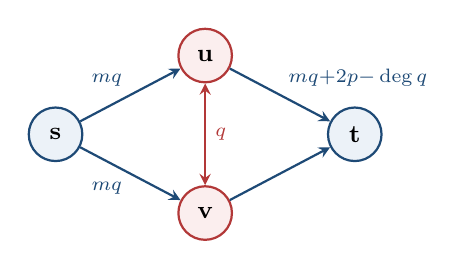
\begin{tikzpicture}[
    st/.style={circle, draw=accent, thick, fill=softbg, minimum size=0.68cm, font=\small\bfseries},
    nd/.style={circle, draw=memberred, thick, fill=softred, minimum size=0.68cm, font=\small\bfseries},
    arr/.style={->, >=stealth, thick, color=accent},
    bi/.style={<->, >=stealth, thick, color=memberred}
]
\node[st] (s) at (0,0) {s};
\node[nd] (u) at (1.9,1.0) {u};
\node[nd] (v) at (1.9,-1.0) {v};
\node[st] (t) at (3.8,0) {t};
\draw[arr] (s) -- node[above left=-1pt,font=\scriptsize] {$mq$} (u);
\draw[arr] (s) -- node[below left=-1pt,font=\scriptsize] {$mq$} (v);
\draw[arr] (u) -- node[above right=-1pt,font=\scriptsize] {$mq{+}2p{-}\deg q$} (t);
\draw[arr] (v) -- (t);
\draw[bi]  (u) -- node[right,font=\scriptsize] {$q$} (v);
\end{tikzpicture}
\end{column}
\end{columns}

\vspace{0.35cm}
\textbf{Lemma.} $\text{cut}(\{s\} \cup S) = mnq + 2\bigl(p|S| - q|E(S)|\bigr)$, because $\sum_{v \in S} \deg v = 2|E(S)| + \partial S$ and the boundary terms cancel.
\end{frame}

% ========================== SLIDE 17 ==========================
\begin{frame}{Proof: reduction and iteration are exact \memberbadge{Shatadeep De}}
\textbf{Theorem 1.} A minimum cut minimises $p|S| - q|E(S)|$. This is negative iff some $S$ has $\rho(S) > p/q$, and then the min-cut side is such a set.

\vspace{0.25cm}
\textbf{Theorem 2 (Dinkelbach, no binary search).} Start from the greedy density. Replace $p/q$ by the density of the set found until no denser set exists. The result is \textbf{optimal}:
\begin{itemize}
\setlength{\itemsep}{0.3em}
\item each round strictly increases $p/q$ or certifies optimality;
\item densities lie in the finite set $\{a/b : a \le m,\; b \le n\}$, so the rounds end;
\item integer capacities mean no rounding errors.
\end{itemize}

\vspace{0.25cm}
\textbf{Pruning.} By the core-degree lemma, $S^*$ lies in the $\lceil \rho_{\text{greedy}} \rceil$-core, so the network is built only on that core.
\end{frame}

% ========================== SLIDE 18 ==========================
\begin{frame}{Evaluation harness \memberbadge{Shatadeep De}}
\begin{itemize}
\setlength{\itemsep}{0.45em}
\item Scored \textbf{per transfer} against the ``Is Laundering'' label: precision, recall, $F_1$.
\item Recall is measured against \emph{all} labels, so one pattern detector cannot reach $1.0$. Self-loop labels are excluded.
\item Running time is measured on the first $25/50/75/100\,\%$ of transfers in time order.
\item The union row combines the pattern detectors. Dense sets are reported separately.
\end{itemize}

\vspace{0.15cm}
{\ttfamily ./aml evaluate data/HI-Small\_Trans.csv > docs/results.md}

\vspace{0.25cm}
\textbf{Tests:} \textbf{2000} random networks (max flow = brute-force min cut) and \textbf{3000} random graphs (exact = optimum over all subsets, with and without pruning; exact beat greedy on 79). Scores are checked by hand, plus an end-to-end synthetic run.
\end{frame}

% ========================== SLIDE 19 ==========================
\begin{frame}{Verification \& synthetic sanity run \memberbadge{Shatadeep De}}
\begin{columns}[T,onlytextwidth]
\begin{column}{0.40\textwidth}
\textbf{Verification}\\
72 checks, 0 failures\\
14\,400 random instances vs brute force\\
\texttt{clang++}, \texttt{g++}, ASan and UBSan

\vspace{0.5cm}
\textbf{Synthetic sanity run}\\
200k transfers, 20k accounts, planted patterns.\\
\emph{Pipeline check, not detection results.}
\end{column}
\begin{column}{0.58\textwidth}
\centering
\footnotesize
\setlength{\tabcolsep}{4.5pt}
\begin{tabular}{@{}lrrr@{}}
\toprule
\textbf{Detector (Synthetic 200k)} & \textbf{Prec.} & \textbf{Recall} & \textbf{Time (s)} \\
\midrule
Temporal cycles & 0.42 & 0.15 & 0.18 \\
Fan-out & 0.47 & 0.27 & 0.005 \\
Fan-in & 0.47 & 0.27 & 0.003 \\
Pass-through chains & 0.66 & 0.32 & 0.03 \\
Exact densest & 0.006 & 1.00 & 0.07 \\
\midrule
\textbf{Union of patterns} & \textbf{0.47} & \textbf{0.86} & \textbf{0.21} \\
\bottomrule
\end{tabular}
\end{column}
\end{columns}
\end{frame}

% ========================== SLIDE 20 ==========================
\begin{frame}{Results on IBM \texttt{HI-Small\_Trans.csv} \memberbadge{Shatadeep De}}
{\footnotesize\textbf{515\,088} accounts, \textbf{5\,078\,345} transfers (5\,166 non-self-loop laundering labels, base rate $0.115\%$), load 3.60\,s, SCC 0.12\,s.}

\vspace{0.18cm}
\centering
{\scriptsize
\setlength{\tabcolsep}{5.5pt}
\begin{tabular}{@{}lrrrrrrl@{}}
\toprule
\textbf{Detector} & \textbf{Flagged} & \textbf{TP} & \textbf{Prec.} & \textbf{Recall} & \textbf{$F_1$} & \textbf{Time (s)} & \textbf{Notes} \\
\midrule
Temporal cycles & 8\,592 & 531 & 0.0618 & 0.1028 & 0.0772 & 1.907 & 11\,959 cycles \\
Fan-out & 1\,169\,117 & 1\,338 & 0.0011 & 0.2590 & 0.0023 & 0.094 & 13\,443 centres \\
Fan-in & 102\,873 & 1\,021 & 0.0099 & 0.1976 & 0.0189 & 0.100 & 6\,906 centres \\
Pass-through chains & 8\,261 & 59 & 0.0071 & 0.0114 & 0.0088 & 1.759 & longest chain 4 \\
\textbf{Max $k$-core} & \textbf{115} & \textbf{66} & \textbf{0.5739} & 0.0128 & 0.0250 & 0.335 & $k = 5$ (26 vertices) \\
Greedy densest & 227 & 66 & 0.2907 & 0.0128 & 0.0245 & 0.335 & 54 vertices, $\rho = 3.574$ \\
Exact densest & 321 & 0 & 0.0000 & 0.0000 & 0.0000 & 0.007 & 81 vertices, $\rho = 3.889$, 3 cuts \\
\midrule
\textbf{Union of patterns} & \textbf{1\,277\,262} & \textbf{2\,820} & 0.0022 & \textbf{0.5459} & 0.0044 & \textbf{3.860} & cycles, fans, chains \\
\bottomrule
\end{tabular}
}

\vspace{0.2cm}
\raggedright
\scriptsize
\begin{itemize}
\setlength{\itemsep}{0.2em}
\item \textbf{5-core precision 57.4\%} ($\approx 500\times$ base rate): 66 of 115 flagged transfers are illicit, unlike the uniform synthetic swamp.
\item \textbf{Core pruning} shrinks 515k vertices to 862 ($4$-core); Edmonds-Karp exact min-cut finishes in \textbf{0.007\,s} ($\rho^* = 3.889 > 3.574$).
\item \textbf{Union recall 54.6\%} in 3.86\,s; unconstrained fan-out flags 13\,443 commercial/payroll hubs, motivating amount/format filters.
\end{itemize}
\end{frame}

% ========================== SLIDE 21 ==========================
\begin{frame}{Conclusion}
\begin{itemize}
\setlength{\itemsep}{0.4em}
\item Five laundering structures, each with a \textbf{formal definition}, a \textbf{proof} and a \textbf{complexity bound}.
\item Guarantees: exact (SCC, cycles, fans, chains, densest subgraph) and $\frac{1}{2}$-approximate (greedy).
\item One unified C++17 pipeline with modular staged architecture and strict mathematical guarantees.
\item Verified against brute force (72 checks, 14\,400 random graphs) and benchmarked on 5.08M IBM AML transfers (\texttt{HI-Small\_Trans.csv}): \textbf{54.6\% union recall} in 3.86\,s and \textbf{57.4\% 5-core precision}.
\item Future work: add amount/format thresholds for fans, currency normalization for chains, and iterative dense-group peeling.
\end{itemize}

\vspace{0.35cm}
\centering
{\Large\bfseries\color{accent} Thank you --- questions?}
\end{frame}

\end{document}
